\part{Cifrari perfetti}
\chapter{Introduzione}
I cifrari perfetti sono cifrari che offrono una \underline{\textbf{sicurezza incondizionata}}, proteggono le informazioni con certezza assoluta di fronte a qualsiasi potenza di calcolo. Solo chi è in possesso della chiave può decifrare. Un attacco a forza bruta non può rompere la cifratura (pur avendo risorse computazionali spropositate).

\paragraph{Costo e crittografia di massa} Si paga un caro prezzo nella loro implementazione, infatti questi cifrari sono usati solo in pochi ambiti,
per la crittografia di massa si preferisce avere una sicurezza computazionale scommettendo su $P \neq NP$.

\paragraph{Definizione informale} Questo concetto è stato formalizzato da Shannon (nel 1949, in realtà prima) informalmente un cifrario è perfetto se la sicurezza è garantita qualunque sia l'informazione carpita dal canale.
\section{Formalizzazione del concetto di \emph{cifrario perfetto}}
Abbiamo lo spazio dei messaggi $MSG$ e lo spazio dei crittogrammi $CRITTO$. Abbiamo poi le variabili aleatorie $M \in MSG$, che descrive il comportamento del mittente, e $C \in CRITTO$, che descrive il processo di comunicazione sul canale. \begin{itemize}
	\item Ricorriamo alla teoria della probabilità per definire:
	\begin{itemize}
		\item $P(M=m)$ : probabilità che il mittente voglia spedire il messaggio $m$ al destinatario
		\item$ P(M=m | C=c)$ : probabilità condizionata (a posteriori) che il messaggio inviato sia effettivamente $m$, dato che sul canale transita il crittogramma $c$
	\end{itemize}
\item Si suppone che il crittoanalista conosca tutto il sistema tranne la chiave. Conosce:
\begin{itemize}
	\item distribuzione di probabilità con cui il mittente invia un messaggio
	\item conosce il cifrario
	\item conosce lo spazio delle chiavi K
\end{itemize}
\end{itemize}
\paragraph{Definizione} {Un cifrario è perfetto se} $\forall m \in MSG$, $\forall c \in CRITTO$ vale:
$$ P(M=m  \mid  C=c) = P(M=m) $$
Cioè: la conoscenza di C non ci permette di dire nulla sul messaggio.

\subsection{Esempi di cifrari non perfetti (casi estremi)}
Supponiamo che ci sia un messaggio $\overline{m}$ che il mittente invia con probabilità $0<p<1$.
$$P(M=\overline{m}) = p$$
Cosa succede in assenza dell'uguaglianza alla base della definizione di cifrario?
\paragraph{Esempio estremo 1}  Supponiamo di avere probabilità uguale ad $1$.
$$\exists \overline{m}, \overline{c} : P(M=\bar{m} \mid C=\bar{c}) = 1$$
Il caso è estremo. Con probabilità $1$ sicuramente il messaggio associato al crittogramma $\overline{c}$ è $\overline{m}$, dunque aumenta la nostra conoscenza sul sistema. 

\paragraph{Esempio estremo 2} Supponiamo una situazione dove la probabilità è nulla
$$\exists \overline{c} : P(M=\overline{m} | C=\overline{c}) = 0$$
ci permette di dire che se passa $\overline{c}$ non è stato sicuramente spedito il messaggio $m$. Anche qui la nostra conoscenza aumenta: il sistema non è perfetto!

\paragraph{Quindi} In un cifrario perfetto la conoscenza complessiva del crittoanalista non cambia dopo che è stato osservato un crittogramma in transito:
\[\boxed{\text{$m$ e $c$ sono del tutto scorrelati, c appare essere una sequenza casuale}}\]

\section{Teorema di Shannon}
\emph{In un cifrario perfetto il numero delle chiavi deve essere maggiore o uguale al numero dei messaggi possibili}
\paragraph{Dimostrazione}Vogliamo dimostrare che $N_k \geq N_m$
\begin{align*} 
	N_m &= \#\{m \in MSG : P(M=m)>0\}\,\,\,\,\,\,\text{Num. dei messaggi possibili}\\
	N_k &= \#\{\text{insieme delle chiavi}\}
\end{align*}
Supponiamo per assurdo che $N_k < N_m$, e prendiamo un crittogramma $c$ tale $$P(C=c)>0$$Cerchiamo di contare quanti messaggi corrispondono a questo crittogramma.
\begin{itemize}
	\item Supponiamo che corrispondano $S$ messaggi. Essi sono i messaggi che posso ottenere decifrando $c$ con tutte le chiavi possibili. Decifro con la chiave $k1$ e ottengo $m1$, decifro con la chiave $k2$ e trovo $m2$, decifro con la chiave $k3$ e ottengo sempre $m2$ (non lo posso escludere), e così via...
	\begin{center}
		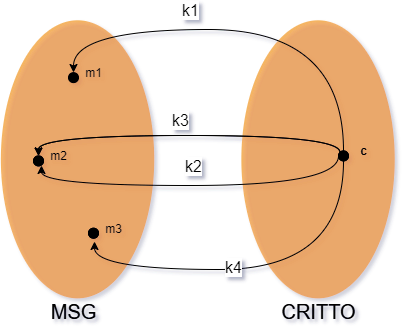
\includegraphics[width = 250pt]{images/Shannon_proof.png}
	\end{center}
	\item Si ha necessariamente $S \leq N_k$ (posso ottenere al più $N_k$ messaggi, non di più).
	\item Poichè abbiamo iniziato con l'ipotesi $N_k < N_m$ otteniamo
	$$S \leq N_k < N_m$$
	quindi
	$$S < N_m$$
	Il numero di messaggi associati al crittogramma $c$ ($S$) è strettamente minore del numero di messaggi possibili.
	\item Appurato che  $S < N_m$ affermiamo che deve esistere un messaggio $m$ con probabilità $P(M=m)>0$ tale che
	$$ P(M=m \mid C=c) = 0 $$
	decifrando $c$ esisterà un $m$ che sicuramente non è il messaggio.
	\item \textbf{Inferisco della conoscenza, quindi contraddico il cifrario perfetto}. Ne deriva quindi che $N_k \geq N_m$. Per usare un cifrario perfetto mi serve quindi una chiave lunghissima!
\end{itemize} 
$\hfill\blacksquare$

\chapter{\emph{One-Time Pad}}
\begin{framed}
	\noindent \textbf{Domanda da esame}. Qual è lo svantaggio principale del cifrario One-Time Pad?
\end{framed} 
\section{Cifratura e decifratura}
Il \emph{One-Time Pad} è un cifrario precedente Shannon, simile ad un Vigenère con chiave lunga quanto il messaggio ma su un alfabeto binario. Nasce nel 1917 da Mauborge e Vernam. \emph{Pad} significa \emph{blocco}, \emph{One-Time} poichè la chiave può essere utilizzata una sola volta.

\paragraph{Ragionamento} Come alfabeto si usa \{0, 1\}. MSG, CRITTO, KEY sono spazi delle sequenze binarie e l'algoritmo di cifratura è noto a tutti ed è lo XOR (somma modulo 2). Supponiamo quindi $m, k \in \{0, 1\}^{n}, n > 0$:
\begin{align*}
	c &= C(m, k) = m \oplus k\\
	 m &= D(c, k) = c \oplus k
\end{align*}

\paragraph{Esempio} Dato $n=5, m=10110, k=01011$ otteniamo
$$c=11101$$
Se io riapplico nuovamente lo XOR ottengo di nuovo
$$m=10110$$
Questo ci torna poichè
$$m = c \oplus k = m \oplus k \oplus k = m \oplus 0 = m$$
\paragraph{Necessità di cambiare la chiave} La chiave deve essere cambiata frequentemente. Supponiamo di non  farlo
\begin{align*}
	c_1 = m_1 \oplus k
	&&
	c_2 = m_2 \oplus k
\end{align*}
Proviamo a fare il seguente calcolo
$$ c_1 \oplus c_2 = m_1 \oplus k \oplus m_2 \oplus k = m_1 \oplus m_2 $$
non ottengo la chiave, ma so che l'operatore XOR restituisce lo zero se due caratteri sono uguali. Il crittoanalista ha imparato qualcosa di nuovo. 
\paragraph{Sicurezza} L'unica informazione ottenibile dal one-time-pad è \textbf{la lunghezza del messaggio}. La sicurezza del One-Time Pad non è computazionale: l'attacco forza bruta non ha alcun senso perchè da tutte le chiavi possibili otteniamo un vasto insieme di messaggi possibili. Mittente e destinatario, a volte, si mandano messaggi privi di senso per rafforzare la sicurezza.





\section{Teorema su \emph{One-time pad} perfetto e minimale}
\emph{One-Time Pad} è un cifrario perfetto e minimale (usa un numero minimo di chiavi) se:
\begin{itemize}
    \item tutti i messaggi hanno lunghezza $n$, se più corti li paddo, se più lunghi li divido in blocchi;
    \item tutte le sequenze di $n$ bit hanno probabilità maggiore di zero di essere inviate (tutte le sequenze di bit sono messaggi, ogni tanto mittente e destinatario si scambiano sequenze prive di significato);
    \item si usano chiavi scelte perfettamente a caso per ogni messaggio.
\end{itemize}
Chiaramente la cosa è complessa: la chiave deve essere lunga quanto il messaggio e deve essere cambiata ogni volta.
\begin{framed}
\noindent Si ricordi la definizione di probabilità condizionata:
$$ P(M=m \mid C=c) \triangleq \frac{P(M=m\text{ e }C=c)}{P(C=c)} $$
Al numeratore abbiamo la probabilità che entrambi gli eventi siano avvenuti: che Alice invii il messaggio $m$ e che l'abbia cifrato ottenendo il crittogramma $c$. Si divide per la probabilità che stia transitando $c$ sul canale di comunicazione.
\end{framed} 
\begin{framed}
	\noindent \textbf{Domanda da esame}. Spiegare con precisione matematica e proprietà di linguaggio perché il cifrario One-Time Pad su messaggi di $n$ bit non può essere ritenuto perfetto se la chiave non è scelta perfettamente a caso
\end{framed}
\paragraph{Dimostrazione perfettezza}
\begin{itemize}
	\item \textbf{Tesi}. La tesi è la definizione di cifrario perfetto:
	$$ \forall m \in MSG, \forall c \in CRITTO $$
	$$ P(M=m \mid C=c) = P(M=m) $$
	\item Stimiamo il numeratore. Dato un messaggio $m$ vogliamo ottenere un crittogramma $c$: per le proprietà dello XOR esiste una sola chiave $k$ in grado di farmi ottenere $c$ a partire da $m$
	$$ \exists! \, k \in \text{KEY}: m \oplus k = c $$
	Segue che la probabilità di ottenere il crittogramma $c$ dal messaggio $m$ è pari alla probabilità di scegliere casualmente la chiave $k$: $\frac{1}{2^n}$ (formulina già trovata, quando abbiamo introdotto la casualità)

	$$\forall c \in \text{CRITTO}\,\,P(C=c)=\frac{1}{2^n}$$
	Nella formula non abbiamo alcuna dipendenza della probabilità dal messaggio (si pensi all'ipotesi 3 del teorema), quindi possiamo scrivere la probabilità nel seguente modo
	$$ P(C=c\text{ e }M=m) = P(M=m) \cdot P(C=c) $$
	\item Prendiamo la definizione di probabilità condizionata e sostituiamo
	$$
	P(M=m \mid C=c) = \frac{P(M=m\text{ e }C=c)}{P(C=c)} = \frac{P(M=m) \cdot \cancel{P(C=c)}}{\cancel{P(C=c)}}
	$$
	siamo arrivati alla definizione di cifrario perfetto!
\end{itemize}
$\hfill\blacksquare$






\paragraph{Dimostrazione minimale}
Sappiamo da Shannon che il numero delle chiavi deve essere maggiore o uguale rispetto al numero dei messaggi $$N_k \geq N_m$$ ma nel one-time pad su lunghezza $n$ ho $2^n$ messaggi possibili, e $2^n$ crittogrammi possibili
$$N_k = N_m= N_{CRITTO} = 2^n$$
Anche le chiavi sono sequenze di bit e ne uso il numero minore possibile. Ricordiamo che tutte le sequenze di $n$ bit sono messaggi possibili: l'attacco forza bruta non ha senso.

$\hfill\blacksquare$


\section{Riduzione della dimensione della chiave}
Cerchiamo di ridurre la dimensione delle chiavi. Pensiamo alla lingua inglese, dove i messaggi significativi sono solo $\alpha^{n}$ con $\alpha = 1.1$
$$\alpha^n << 2^n$$
Poniamo $N_m = \alpha^n$ dato che $N_k = 2^t \geq N_m = \alpha^n$. Vogliamo individuare il numero di bit $t$, necessari affinchè 
\begin{align*}
	2^t \geq \alpha^n \longrightarrow t \cdot \log_2 2 \geq \log_2\alpha^n &= n \cdot \log_2\alpha \\ t \geq \log_2\alpha^n &= n \cdot \log_2\alpha \longrightarrow t \geq 0.12 \cdot n
\end{align*}
Posso quindi usare chiavi molto più corte: $\approx 10\%$ di $n$.

\paragraph{Come fare?} Genero i $t$ bit randomicamente e li estendo in maniera deterministica su $n$ bit (funzione che dato in ingresso una sequenza su $t$ bit mi restituisce una sequenza su $n$ bit, sempre lo stesso output con lo stesso input).
Dobbiamo però metterci al riparo dall'attacco forza bruta: è fondamentale che coppie diverse di
$(m, k)$ producano lo stesso crittogramma. Per far ciò il $\#(m, k)$ deve essere di molto maggiore di $\#CRITTO$:
$$ \alpha^n \cdot 2^t >> 2^n \xrightarrow{} t >> 0.88n$$
In definitiva ci serve $t >> 88\%n$ quindi non si ha una grande compressione della chiave.
